\documentclass[conference]{IEEEtran}
\IEEEoverridecommandlockouts
\usepackage[utf8]{inputenc}
\usepackage[T1]{fontenc}
\usepackage{cite}
\usepackage{amsmath,amssymb,amsfonts}
\usepackage{algorithmic}
\usepackage{graphicx}
\usepackage{textcomp}
\usepackage{xcolor}
\usepackage{booktabs}
\usepackage{hyperref}
\def\BibTeX{{\rm B\kern-.05em{\sc i\kern-.025em b}\kern-.08em
    T\kern-.1667em\lower.7ex\hbox{E}\kern-.125emX}}

\begin{document}

\title{Correlation between General Health and Mental Health Based on Housing Situation for Indigenous Populations\thanks{Course project for Data Analysis with Python, Winter 2026, Algoma University.}}

\author{
\IEEEauthorblockN{Dylan Luong}
\IEEEauthorblockA{\textit{Algoma University} \\
Student ID: 5150921 \\
Brampton, Canada}
\and
\IEEEauthorblockN{Iman Fatima Ghani}
\IEEEauthorblockA{\textit{Algoma University} \\
Student ID: 5152246 \\
Brampton, Canada}
\and
\IEEEauthorblockN{Jehosua Alan Joya Venegas}
\IEEEauthorblockA{\textit{Algoma University} \\
Student ID: 5149910 \\
Brampton, Canada}
\and
\IEEEauthorblockN{Saurodeep Majumdar}
\IEEEauthorblockA{\textit{Algoma University} \\
Student ID: 5153010 \\
Brampton, Canada}
}

\maketitle

\begin{abstract}
This paper presents a descriptive Python dashboard built from Statistics Canada Table 41-10-0080-01 on general health, mental health, and housing conditions among Indigenous populations in Canada. The workflow parses a wide-format government export into 10,400 long-form records, excludes suppressed rows marked \texttt{F}, retains estimated rows marked \texttt{E} with caution, and recomputes within-condition shares from \texttt{Number of persons} values to support clearer comparisons. The final dashboard is organized as a narrative with a national snapshot, a regional crowding map, repair-needs and health views, crowding and health views, and an exploration-story section that documents how the analysis evolved from weekly exploratory work into the final presentation. The strongest findings show that fair-or-poor health becomes much more common as repair needs worsen, while severe crowding is regionally concentrated, especially in Nunavut. Overall, the project demonstrates how Python can turn a difficult published table into an interpretable, reproducible, and presentation-ready visual analysis.
\end{abstract}

\begin{IEEEkeywords}
Indigenous health, housing conditions, crowding, repair needs, Statistics Canada, dashboard, Python
\end{IEEEkeywords}

\section{Introduction}

\IEEEPARstart{H}{ousing} is widely recognized as a social determinant of health because conditions such as overcrowding, structural damage, and inadequate maintenance can affect safety, stress, privacy, and everyday well-being \cite{who2018}. This relationship is especially important for Indigenous populations in Canada, where housing conditions are connected to broader structural inequalities and geographic differences in access, infrastructure, and living conditions \cite{nccih2017}. To study this issue using official published evidence, this paper analyzes Statistics Canada Table 41-10-0080-01, \emph{General health and mental health by housing situation, First Nations people living off reserve, M\'etis and Inuit}, based on the 2022 Indigenous Peoples Survey (IPS) \cite{statcantable,statcanips}.

This paper presents a descriptive Python-based dashboard that transforms a difficult wide-format government table into a reproducible visual analysis of general health, mental health, repair needs, crowding, and regional variation. The goal is not to estimate causation, but to show how published health outcomes are distributed across housing conditions and geographies in a way that is transparent and interpretable. The final dashboard is organized as a narrative, moving from a national snapshot to a regional map and then to repair-needs and crowding views, while also including an exploration-story section that explains how the weekly notebook work evolved into the final presentation.

The paper contributes the following:
\begin{itemize}
\item \textbf{A reproducible parsing and cleaning workflow} that converts the Statistics Canada export into 10,400 long-form records, standardizes labels, excludes suppressed \texttt{F} rows, and retains estimated \texttt{E} rows with caution.
\item \textbf{A dashboard-centered analytical model} that recomputes within-condition health shares from \texttt{Number of persons} values, allowing clearer comparisons across repair conditions and crowding levels than the raw published percentages alone.
\item \textbf{An evidence-based descriptive presentation} showing that fair-or-poor health becomes much more common as repair needs worsen, and that severe crowding is strongly concentrated in northern geographies such as Nunavut.
\end{itemize}

The remainder of this paper is organized as follows. Section~II reviews the housing-and-health context motivating the analysis. Section~III describes the dataset and the parsing workflow used to build the analytical table. Section~IV explains the structure of the final dashboard, including the exploration-story component. Section~V presents the main descriptive results from the national, regional, repair-needs, and crowding views. Section~VI discusses interpretation and limitations. Section~VII concludes with the main findings and the value of the final dashboard as a course project deliverable.

\section{Background}

Housing and health are closely connected in public health research. The World Health Organization has emphasized that poor housing conditions can increase health risks through structural problems, exposure, instability, and psychosocial stress \cite{who2018}. Housing shapes safety, comfort, privacy, and everyday well-being, which is why it is often discussed as a social determinant of health rather than simply as a consumer good.

The relationship is especially relevant when studying mental health. Housing stress, overcrowding, and inadequate repair conditions can produce chronic stress, reduce privacy, and affect family dynamics. Research on housing stress and affordability has shown meaningful associations between poor housing conditions and psychological distress \cite{bentley2012}. These findings suggest that when general health and mental health are studied together, housing conditions can help explain differences in how people report their well-being.

For Indigenous populations in Canada, this issue has both public health and social significance. The National Collaborating Centre for Indigenous Health describes housing as a key determinant of First Nations, Inuit, and M\'etis health, noting that quality, affordability, safety, and crowding affect both physical and emotional well-being \cite{nccih2017}. In this context, a descriptive data analysis project is useful because it makes patterns in official national data easier to interpret and communicate.

\section{Dataset and Methods}

\subsection{Dataset Structure}

The dataset used in this project is the local file \texttt{4110008001\_databaseLoadingData.csv}, downloaded from Statistics Canada Table 41-10-0080-01:

\begin{center}
\url{https://www150.statcan.gc.ca/t1/tbl1/en/tv.action?pid=4110008001}
\end{center}

The updated version of the file used in the dashboard is not a simple flat CSV. It is a wide-format export that contains metadata rows, repeated year labels, region columns, and multiple statistics for each housing and health category. Because of that layout, the first step of the workflow was to build a parser that converts the published table into a long analytical format.

The parsed dataset contains 10,400 rows and the following main fields:
\texttt{Geography},
\texttt{Indigenous identity},
\texttt{Age group},
\texttt{Gender},
\texttt{Overall health},
\texttt{Housing - Needs repairs},
\texttt{Persons per room (crowding)},
\texttt{Statistics},
\texttt{VALUE}, and
\texttt{STATUS}.

The table includes four types of published statistics: number of persons, percent, low 95\% confidence interval, and high 95\% confidence interval. The \texttt{STATUS} field is also important. Rows marked \texttt{F} are too unreliable to publish and do not contain a usable value. Rows marked \texttt{E} are estimates that should be interpreted with caution. In the parsed file, 5,270 rows are flagged \texttt{F} and 285 rows are flagged \texttt{E}. In the final dashboard, \texttt{F} rows are excluded, while \texttt{E} rows are retained with caution.

One major difference between the refreshed file and the earlier working version is the structure of the demographic fields. In the updated file, geography is richly represented, but \texttt{Indigenous identity}, \texttt{Age group}, and \texttt{Gender} appear as totals in the published layout used for the final dashboard. That means the strongest comparisons available in this version of the table are geographic and housing-based rather than subgroup comparisons by identity, age, or gender.

\subsection{Analytical Workflow}

The analytical logic is implemented in \texttt{analysis\_utils.py}, while \texttt{app.py} uses those functions to render the dashboard. The workflow can be summarized in five steps:

\begin{enumerate}
    \item parse the Statistics Canada export into long-form rows;
    \item normalize text labels and remove suppressed \texttt{F} rows from analytical views;
    \item select the slices needed for the dashboard;
    \item recompute within-condition health shares from \texttt{Number of persons};
    \item organize the results into a narrative dashboard.
\end{enumerate}

Another important methodological choice concerns how the health comparisons are calculated. Some of the published percentages in the raw table are normalized within health categories, which makes them less useful for directly answering the question of how health composition changes across housing conditions. To make that comparison clearer, the dashboard uses \texttt{Number of persons} rows and recomputes within-condition shares in Python. This produces interpretable comparisons such as the share of people reporting excellent or very good, good, or fair or poor health within each repair condition and within each crowding level.

\section{Dashboard Structure and Exploration Story}

The final dashboard is the presentation layer of the project, and it is organized in the same order that we plan to present it:

\begin{itemize}
    \item Guide
    \item Exploration Story
    \item National Snapshot
    \item Regional Map
    \item Repair Needs and Health
    \item Crowding and Health
    \item Data
\end{itemize}

The \textit{Exploration Story} section is one of the most important additions to the final dashboard because it connects the weekly notebook work to the polished presentation. Instead of only showing final charts, the dashboard explains how the exploration unfolded and why certain design choices were made.

This section highlights three discoveries from the data exploration phase. First, the published file had to be parsed before it could be analyzed. The wide Statistics Canada export was converted into 10,400 long-form rows covering 13 geographies. Second, quality flags had to be handled explicitly: rows marked \texttt{F} were excluded, while rows marked \texttt{E} were retained with caution. Third, raw percentages were not always enough for the final story. During exploration, some raw \texttt{Percent} rows returned values such as 100.0 across all repair categories for the same health slice. That result was technically published, but it was not useful for answering the project question. This is why the final dashboard relies on \texttt{Number of persons} and recomputed within-condition shares.

That transition from exploration to interpretation is visible in the final dashboard. The exploration stage revealed that fair-or-poor mental health rises from 23.9\% in regular-maintenance homes to 43.0\% in major-repairs homes, while severe crowding in the Canada total is 3.5\% but reaches 31.4\% in Nunavut. These are exactly the kinds of patterns that survived the exploration stage and became central to the final presentation.

\section{Results}

\subsection{National Snapshot}

The first dashboard section establishes the national baseline for the published population. The Canada total in the table is 1,077,810 people. The dashboard shows two important housing summaries.

\begin{figure}[htbp]
\centering
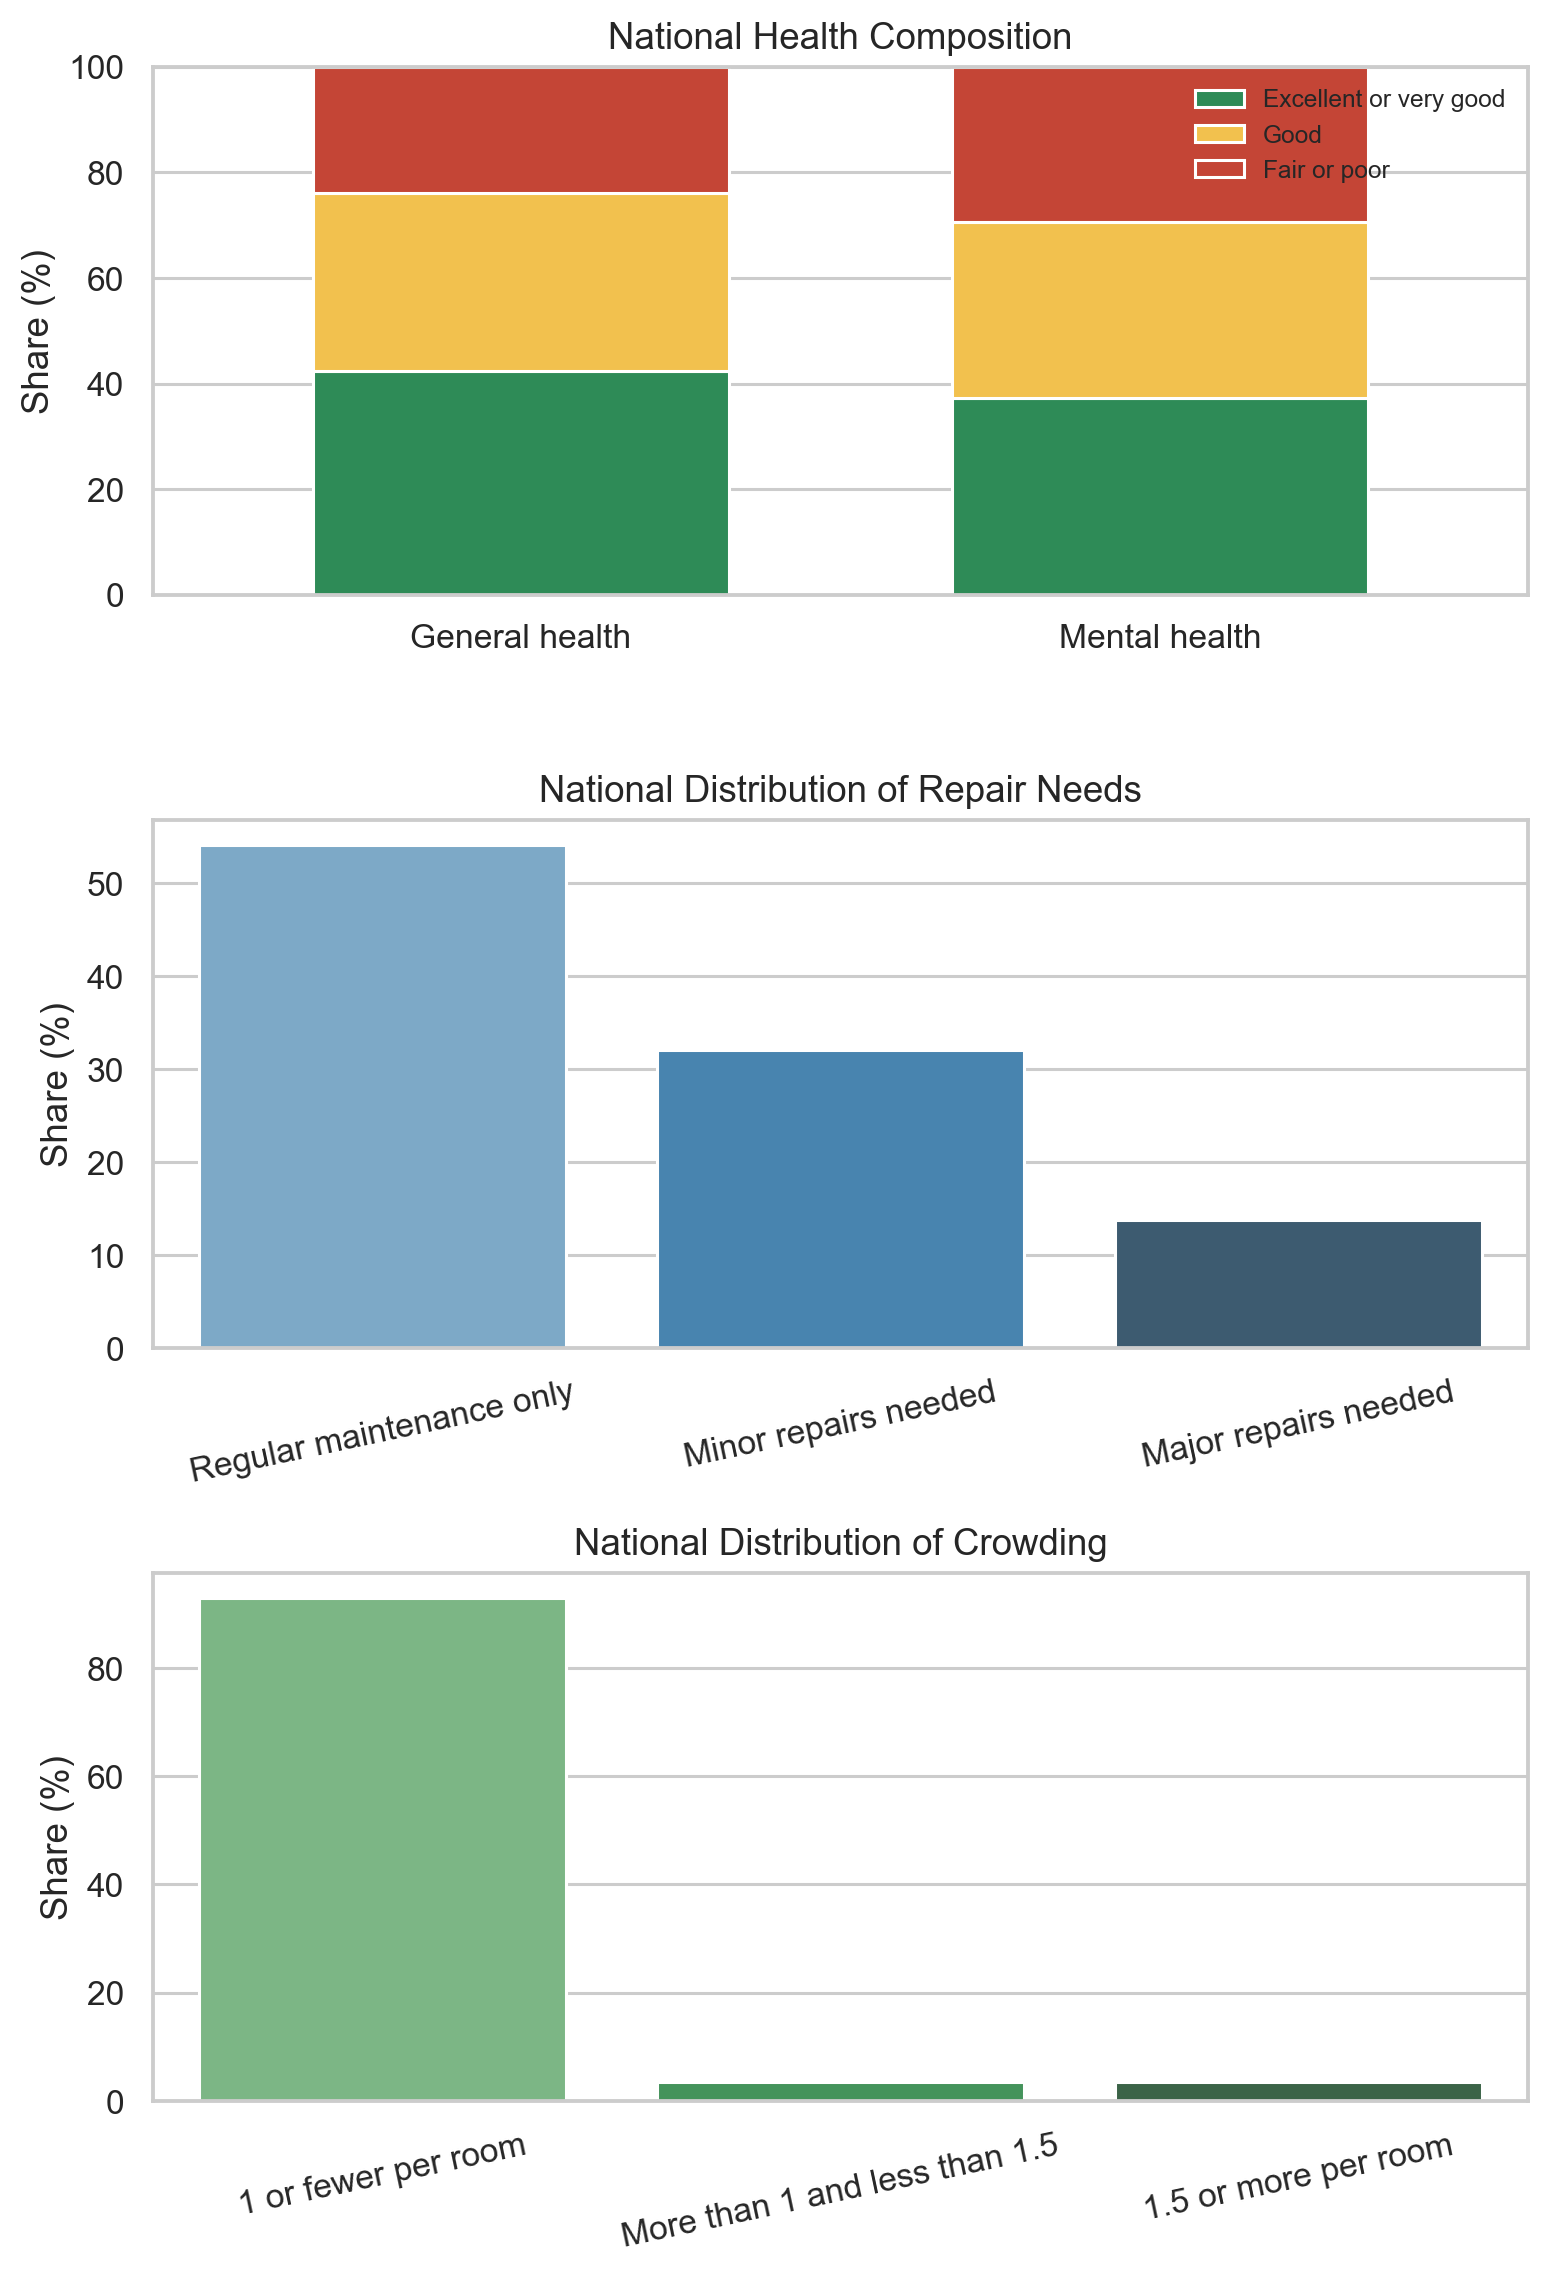
\includegraphics[width=0.95\columnwidth]{national_snapshot.png}
\caption{National snapshot of health composition, repair needs, and crowding in the Canada total.}
\label{fig:national_snapshot}
\end{figure}

For repair needs:
\begin{itemize}
    \item 54.2\% are in dwellings needing only regular maintenance;
    \item 32.1\% are in dwellings needing minor repairs;
    \item 13.7\% are in dwellings needing major repairs.
\end{itemize}

For crowding:
\begin{itemize}
    \item 92.9\% are in dwellings with one person or fewer per room;
    \item 3.5\% are in dwellings with more than one but less than 1.5 persons per room;
    \item 3.5\% are in dwellings with 1.5 persons or more per room.
\end{itemize}

The dashboard also compares the national composition of general health and mental health. For general health, 42.3\% report excellent or very good health and 23.9\% report fair or poor health. For mental health, 37.2\% report excellent or very good health and 29.5\% report fair or poor mental health. This means the national baseline is already somewhat more fragile for mental health than for general health.

\subsection{Regional Map}

The updated Statistics Canada file introduced regional, provincial, and territorial geography into the dashboard. This allowed the addition of a real regional map rather than a placeholder visualization.

\begin{figure}[htbp]
\centering
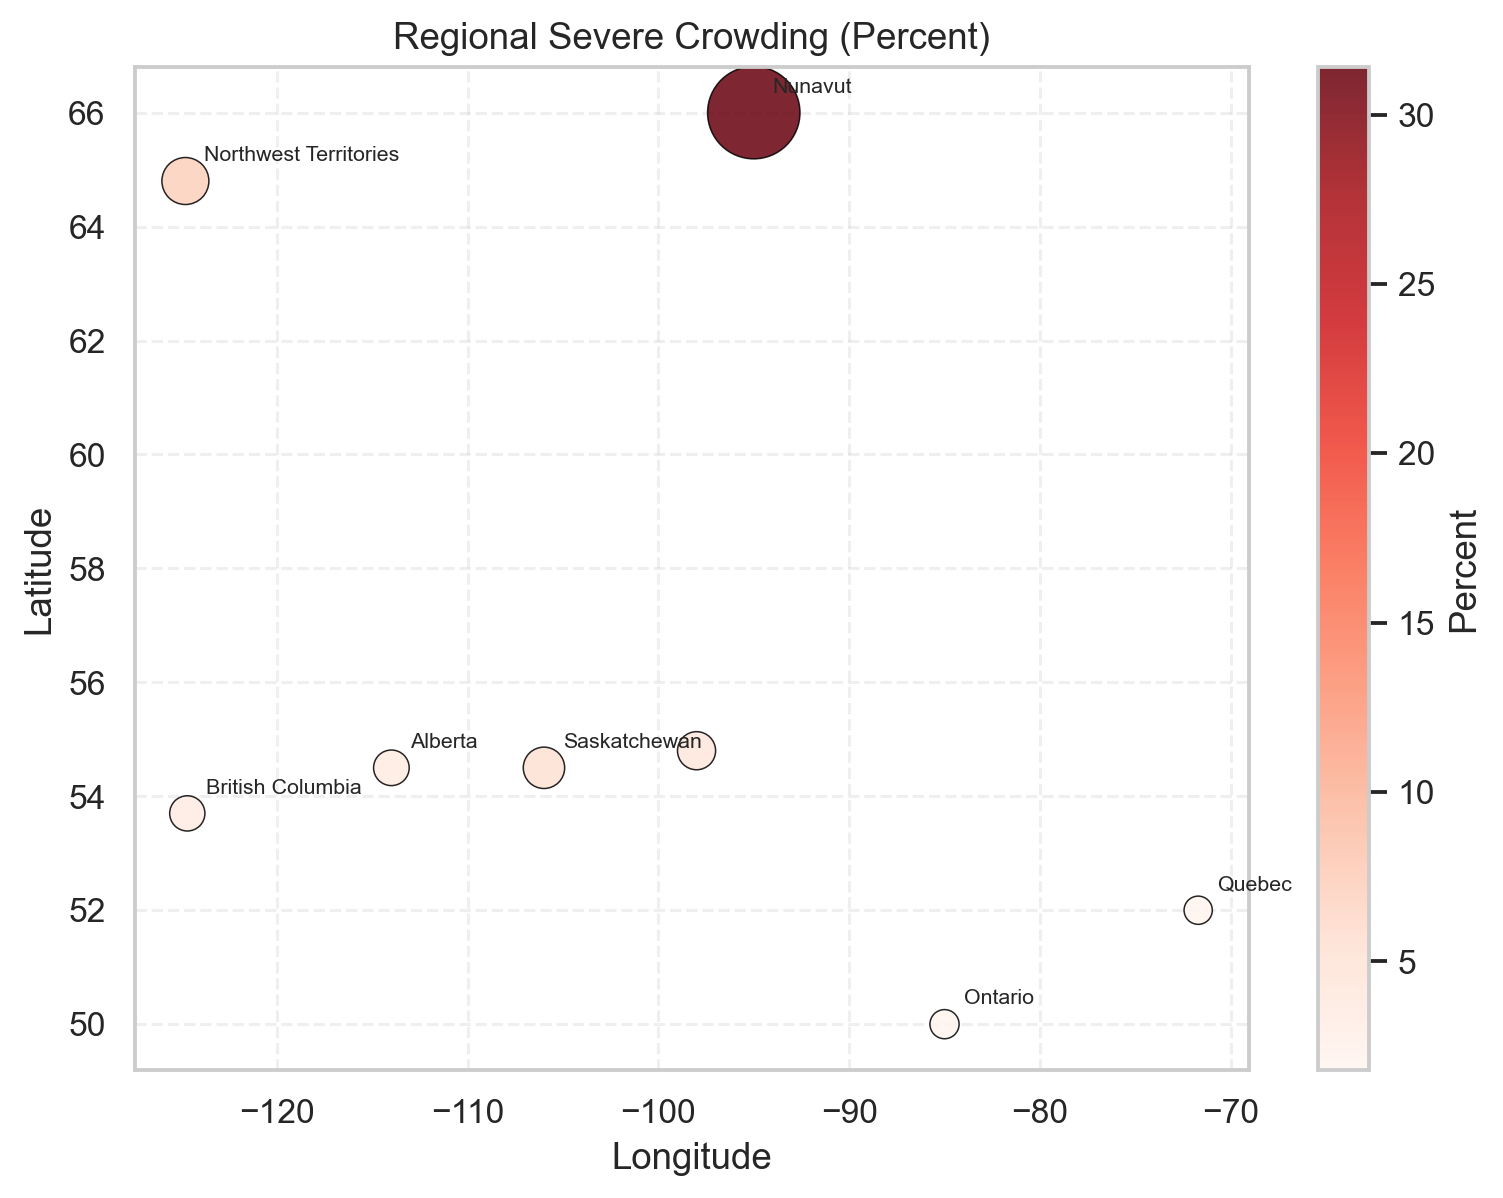
\includegraphics[width=\columnwidth]{regional_map.png}
\caption{Regional distribution of severe crowding across Canada, with Nunavut standing out clearly.}
\label{fig:regional_map}
\end{figure}

The most revealing map setting is:
\begin{itemize}
    \item measure = total self-perceived general health;
    \item crowding category = 1.5 persons or more per room;
    \item statistic = percent.
\end{itemize}

Under that setting, the highest published value appears in Nunavut at 31.4\%. The broader Territories grouping also stands out at 21.3\%, followed by the Northwest Territories at 7.2\%. Most provinces have much lower values, including Ontario at 2.0\%, Quebec at 1.8\%, and the Atlantic provinces at 1.7\%.

This regional contrast is one of the clearest findings in the project. Severe crowding is not distributed evenly across geography. The northern geographies stand out sharply, especially Nunavut. The map also becomes more informative when the user switches from total health to fair-or-poor health categories. For example, fair-or-poor mental health under severe crowding is highest in Nunavut at 34.9\%, followed by the Territories grouping at 20.2\%.

\subsection{Repair Needs and Health}

The strongest relationship in the dashboard appears in the repair-needs section. This section uses \texttt{Number of persons} and recalculates the share of health categories within each repair condition.

\begin{figure}[htbp]
\centering
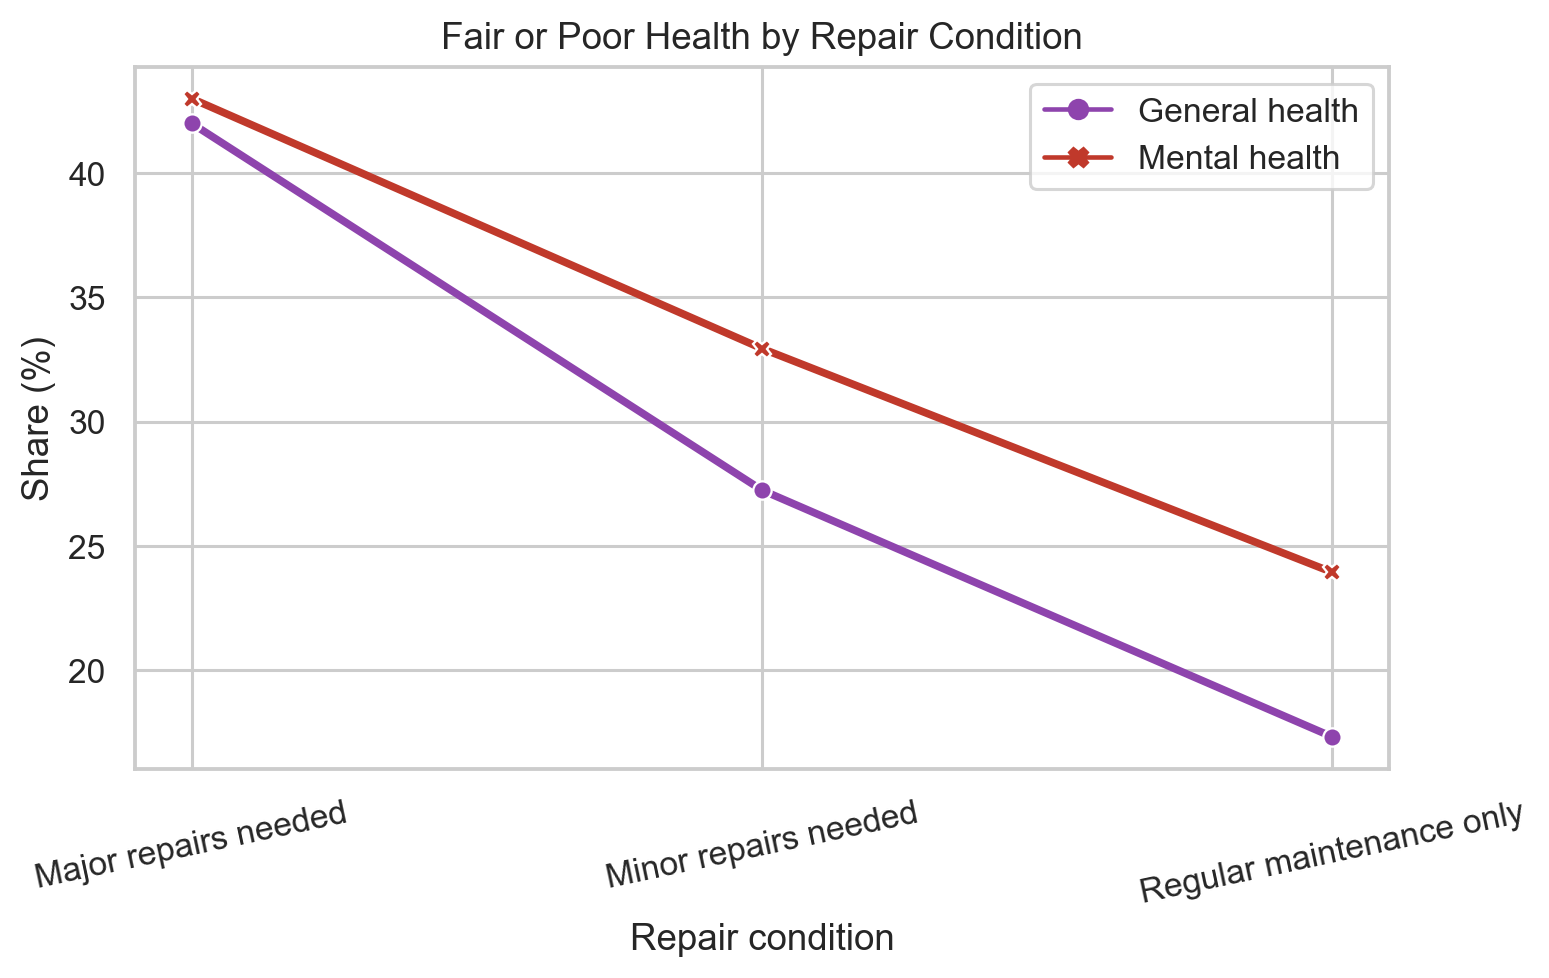
\includegraphics[width=\columnwidth]{repair_needs_chart.png}
\caption{Fair-or-poor health becomes more common as housing repair needs worsen.}
\label{fig:repair_needs}
\end{figure}

For general health, the composition changes substantially as repair needs worsen.

\begin{table}[htbp]
\caption{General health composition by repair condition}
\label{tab:general_repairs}
\centering
\resizebox{\columnwidth}{!}{%
\begin{tabular}{lccc}
\toprule
Repair condition & Excellent or very good & Good & Fair or poor \\
\midrule
Regular maintenance only & 50.4\% & 32.2\% & 17.3\% \\
Minor repairs needed & 35.6\% & 37.1\% & 27.2\% \\
Major repairs needed & 26.1\% & 31.9\% & 42.0\% \\
\bottomrule
\end{tabular}%
}
\end{table}

For mental health, the pattern is just as strong.

\begin{table}[htbp]
\caption{Mental health composition by repair condition}
\label{tab:mental_repairs}
\centering
\resizebox{\columnwidth}{!}{%
\begin{tabular}{lccc}
\toprule
Repair condition & Excellent or very good & Good & Fair or poor \\
\midrule
Regular maintenance only & 43.5\% & 32.5\% & 23.9\% \\
Minor repairs needed & 31.6\% & 35.5\% & 32.9\% \\
Major repairs needed & 25.6\% & 31.4\% & 43.0\% \\
\bottomrule
\end{tabular}%
}
\end{table}

These tables show the clearest headline result of the project: more severe repair needs are associated with worse self-reported health composition, both for general health and for mental health.

\subsection{Crowding and Health}

The crowding section tells a more nuanced story than the repair-needs section. The relationship is still meaningful, but it is not equally strong for general health and mental health.

\begin{figure}[htbp]
\centering
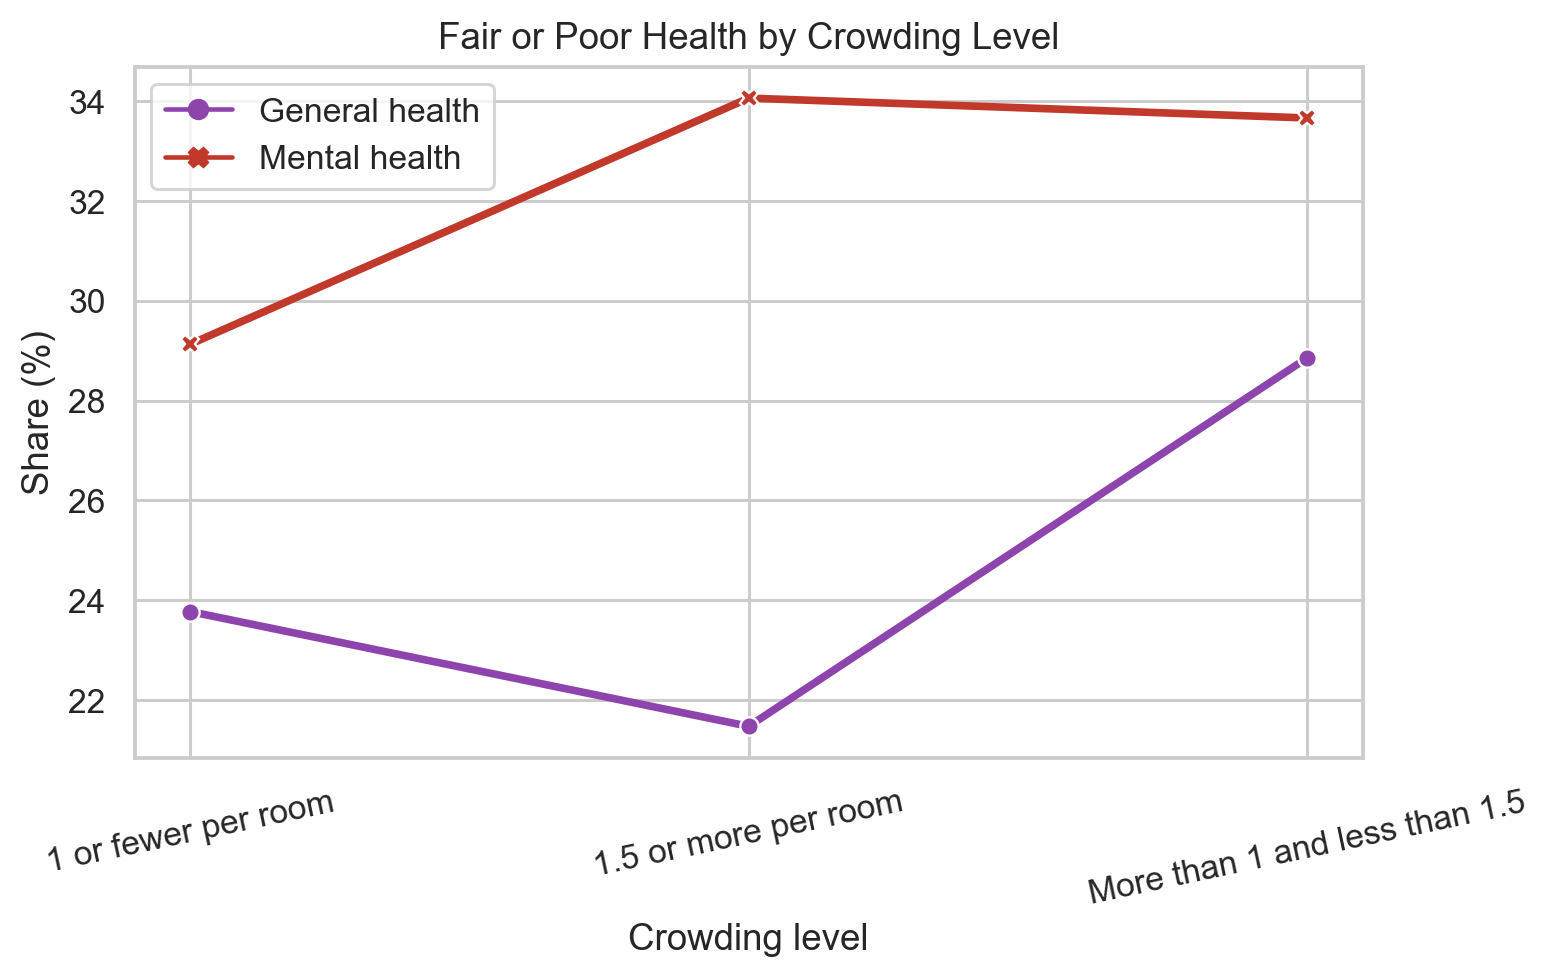
\includegraphics[width=\columnwidth]{crowding_chart.png}
\caption{Crowding has a clearer descriptive relationship with mental health than with general health.}
\label{fig:crowding_health}
\end{figure}

For general health:

\begin{table}[htbp]
\caption{General health composition by crowding level}
\label{tab:general_crowding}
\centering
\resizebox{\columnwidth}{!}{%
\begin{tabular}{lccc}
\toprule
Crowding level & Excellent or very good & Good & Fair or poor \\
\midrule
1 or fewer per room & 42.5\% & 33.7\% & 23.8\% \\
More than 1 and less than 1.5 & 40.3\% & 30.9\% & 28.9\% \\
1.5 or more per room & 40.2\% & 38.3\% & 21.5\% \\
\bottomrule
\end{tabular}%
}
\end{table}

For mental health:

\begin{table}[htbp]
\caption{Mental health composition by crowding level}
\label{tab:mental_crowding}
\centering
\resizebox{\columnwidth}{!}{%
\begin{tabular}{lccc}
\toprule
Crowding level & Excellent or very good & Good & Fair or poor \\
\midrule
1 or fewer per room & 37.8\% & 33.1\% & 29.1\% \\
More than 1 and less than 1.5 & 32.2\% & 34.1\% & 33.7\% \\
1.5 or more per room & 28.2\% & 37.7\% & 34.1\% \\
\bottomrule
\end{tabular}%
}
\end{table}

For mental health, fair-or-poor outcomes rise as crowding increases, while the excellent-or-very-good share falls. The increase is not as large as the repair-needs effect, but it is consistent enough to support the interpretation that crowding is more strongly associated with mental health than with general health in this published table.

\section{Discussion}

The final dashboard supports the broad argument of the project proposal: housing situation is meaningfully related to self-reported health in the Indigenous Peoples Survey data. The evidence is strongest for repair needs. As housing conditions move from regular maintenance to major repairs, the share of fair-or-poor health rises sharply. This is true for both general health and mental health, and the shift is large enough to be visible immediately in the charts.

At the same time, one of the most important outcomes of this project is methodological rather than purely descriptive. The semester made it clear that good results depend on a sequence of practical analytical skills: understanding a dataset before graphing it, cleaning labels carefully, checking what the published percentages actually mean, and selecting the visual form that best answers the research question. Those skills were developed week by week through exploratory notebook work, and they became essential once the team had to move from early trial charts to a polished dashboard.

Crowding contributes a second layer to the story. At the national level, severe crowding is less common than repair needs, but the regional map shows that it is not evenly distributed. The map makes it clear that certain northern geographies, especially Nunavut, stand out strongly. This gives the dashboard a useful geographic dimension that was missing from the earlier working version of the dataset. The crowding-health relationship is also more nuanced than the repair-health relationship. For general health, the pattern is mixed. For mental health, however, the fair-or-poor share increases as crowding becomes more severe. This suggests that mental health may be more sensitive to crowded living conditions in the published data than general health is.

Another important learning from the semester was that reproducibility matters as much as interpretation. Building \texttt{analysis\_utils.py}, parsing the wide-format Statistics Canada file, and consistently applying the same filtering logic forced the project to move beyond one-off notebook exploration. In practice, that meant turning classroom skills in Python, data wrangling, and visualization into a repeatable workflow that could support a final dashboard and a formal report at the same time.

These results should still be interpreted carefully. The project does not establish causation. The data are aggregated and published in table form, not individual-level survey microdata. The dashboard describes patterns in the official Statistics Canada output; it does not estimate causal effects and it does not predict outcomes for individual people or communities. There are also limitations related to published suppression. Rows marked \texttt{F} had to be excluded, and rows marked \texttt{E} were retained with caution. That means some categories remain more uncertain than others. Even so, using the published counts and recalculating within-condition shares produced a more interpretable dashboard than relying only on the raw percentages in the table.

\section{Conclusion}

The report and the dashboard tell the same story. Housing repair needs show the strongest descriptive relationship with worse self-reported health, crowding adds an important second dimension that is especially visible for mental health, and regional comparison shows that severe crowding is concentrated much more heavily in northern geographies such as Nunavut.

More importantly, the final project shows how the skills developed during the semester made this result possible. Early course work emphasized data cleaning, exploratory plotting, interpretation of published values, and the importance of questioning what a visualization is really showing. Those lessons directly shaped the final product. Without that progression, the project would likely have remained a set of disconnected exploratory charts rather than a coherent and defensible dashboard.

In that sense, the project succeeds not only analytically, but also as a reflection of the semester's learning goals. It demonstrates that Python can be used to parse a difficult public dataset, turn exploratory work into a reproducible pipeline, and present the results through a structured visual narrative. The final dashboard therefore serves both as a substantive analysis of housing and health and as evidence of the practical skills gained throughout the course.

\section*{Acknowledgment}

This project uses published data from Statistics Canada's 2022 Indigenous Peoples Survey tables. The dashboard and analysis were developed as part of a course project in Data Analysis with Python. The authors also acknowledge the contextual guidance provided by public health and Indigenous health literature, which helped frame the interpretation of housing as a social determinant of health.

\begin{thebibliography}{00}

\bibitem{bentley2012}
R. Bentley, A. Baker, and K. Mason, ``Housing affordability, housing stress and mental health,'' \emph{BMC Public Health}, vol. 12, no. 1, pp. 1--8, 2012.

\bibitem{statcanips}
Government of Canada, Statistics Canada, ``Indigenous Peoples Survey (IPS),'' Surveys and Statistical Programs, 2024. [Online]. Available: \url{https://www23.statcan.gc.ca/imdb/p2SV.pl?Function=getSurvey&SDDS=3250}

\bibitem{nccih2017}
National Collaborating Centre for Indigenous Health, \emph{Housing as a Social Determinant of First Nations, Inuit and M\'etis Health}, 2017. [Online]. Available: \url{https://www.ccnsa-nccah.ca/docs/determinants/FS-Housing-SDOH2017-EN.pdf}

\bibitem{statcantable}
Statistics Canada, ``Table 41-10-0080-01: General health and mental health by housing situation, First Nations people living off reserve, M\'etis and Inuit,'' 2024. [Online]. Available: \url{https://www150.statcan.gc.ca/t1/tbl1/en/tv.action?pid=4110008001}

\bibitem{who2018}
World Health Organization, \emph{WHO Housing and Health Guidelines}. Geneva, Switzerland: World Health Organization, 2018.

\end{thebibliography}

\end{document}
